En la actualidad, la conectividad y la seguridad de las redes corporativas son pilares fundamentales para garantizar su correcto funcionamiento, es por ello, que la mayoría de las empresas están en un proceso de transformación digital. Por supuesto, aquellas organizaciones con varias sedes requieren de una infraestructura de red eficiente, robusta, escalable y que cuente con una comunicación segura entre ellas.

\vspace{0.5cm}
A medida que la tecnología sigue avanzando y los servicios en línea se vuelven parte esencial del día a día (como ocurre con la telefonía basada en IP, las plataformas en la nube o el acceso remoto a sistemas), se hace cada vez más necesario contar con redes que integren herramientas actuales, por lo que la elección de las tecnologías core adquieren un papel crucial. El objetivo es facilitar la interacción entre ubicaciones en diferentes áreas geográficas, lo cual permite que los datos se transmitan de manera eficiente entre redes y dispositivos. También es 
importante garantizar un tránsito de información ágil y confiable en toda la estructura de red.

\vspace{0.5cm}
La elección de la tecnología de interconexión adecuada depende de varios factores, como el tamaño de la red, el tipo de tráfico que se espera, la latencia o el ancho de banda requerido. Cada una de estas presenta sus propias ventajas y desventajas, y la selección de la más apropiada debe basarse en las necesidades específicas de la organización. Existen diversas tecnologías \cite{conexion_redes_extendidas}, como por ejemplo:
\begin{itemize}
  \item \textbf{ATM (Asynchronous Transfer Mode):} es la conjunción de las redes de conmutación de circuitos y de conmutación de paquetes, también conocida como ``cell relay''. Está basada principalmente en el concepto de conmutación de paquetes, pero con un tamaño fijo, y es capaz de prestar servicios que requieren una velocidad constante o prestaciones de la conmutación de circuitos, todo ello utilizando señalización por canal común.
  \item \textbf{Frame Relay:} es un protocolo WAN de alto rendimiento que funciona en las capas físicas y de enlace de datos del modelo de referencia OSI. Frame Relay reduce los costos de redes a través del uso de menos equipos, menos complejidad y una implementación más fácil. Proporciona un mayor ancho de banda, mejor fiabilidad y resistencia a fallas que las líneas privadas o arrendadas.
  \item \textbf{X.25:} es un estándar de protocolo de la Unión Internacional de Telecomunicaciones, Sector de Estandarización de Telecomunicaciones (ITU-T) para la comunicación WAN que define cómo los dispositivos de usuario y los dispositivos de red establecen y mantienen conexiones.
  \item \textbf{MPLS (Multiprotocol Label Switching):} es una técnica de alto rendimiento para transportar datos en redes de telecomunicaciones, donde ha ido reemplazando a Frame Relay y ATM. MPLS se encarga de dirigir los datos de un nodo de red al siguiente utilizando etiquetas de ruta en lugar de direcciones de red. De esta forma conseguimos agilizar la red, pues los nodos no tienen que desencapsular direcciones de red muy largas y cotejarlas en una tabla de enrutamiento \cite{mpls_elements}.  
  \item \textbf{SD-WAN (Software-Defined Wide Area Network):} es una red de área extensa (WAN) que utiliza tecnología de redes definidas por software, como la comunicación a través de Internet mediante túneles superpuestos que se cifran cuando se destinan a ubicaciones internas de la organización \cite{wikipedia_sdwan}.
  \item \textbf{VPN (Virtual Private Network):} es una tecnología de red que permite una extensión segura de la red de área local (LAN) sobre una red pública o no controlada como Internet. Permite que dispositivos en la red envíe y reciba datos sobre redes compartidas o públicas como si fuera una red privada, con toda la funcionalidad, seguridad y políticas de gestión de una red privada \cite{wikipedia_vpn}.
\end{itemize}

\vspace{0.5cm}
Por lo tanto, el diseño de red es importante a la hora de crear una infraestructura de comunicaciones eficiente,
ya que esta se encarga de definir la estructura física y lógica, como elegir los componentes que se van a
utilizar, las tecnologías de interconexión, etc. La creación de una red bien diseñada no solo garantiza
conectividad, sino que también optimiza el rendimiento, la escalabilidad y la seguridad mediante el
diseño de una red jerárquica.

\section{Objetivos}
El objetivo fundamental de este Trabajo de Fin de Grado es implantar un sistema de comunicaciones unificado que facilite la gestión e integración de servicios, mejorando así la eficiencia y seguridad de las comunicaciones entre las distintas sedes de una empresa. Para ello, se ha tomado como referencia el pliego técnico del expediente \cite{expediente0062020} del Consorcio de Aguas de la Zona Gaditana, el cual plantea una propuesta integral de modernización, equipamiento y mejora de la conectividad del consorcio. No obstante, este trabajo no aborda la totalidad del contenido del pliego, sino que se centra únicamente en el diseño y simulación de determinados aspectos clave de la infraestructura de red. Para alcanzar estos fines, 
se plantean también una serie de objetivos específicos, entre los cuales se encuentran los siguientes:

\begin{itemize}
  \item Diseñar una red de interconexión entre las sedes del consorcio utilizando tecnologías de interconexión modernas y eficientes.
  \item Utilizar herramientas de simulación como GNS3 para validar el diseño y la configuración de la red.
  \item Elección de dispositivos de red adecuados para la infraestructura, incluyendo routers, switches y firewalls.
  \item Crear un esquema de direccionamiento IPv6 para garantizar la escalabilidad y la compatibilidad con las tecnologías actuales.
\end{itemize}

\newpage

\section{Antecedentes}
El Consorcio de Aguas de la Zona Gaditana (CAZG) es una entidad pública, con sede principal en Jerez de la Frontera, que se encarga de gestionar el ciclo integral del agua en la provincia de Cádiz. Su función principal es asegurar el abastecimiento de agua potable y el saneamiento de aguas residuales para la población de la zona. Actualmente, el consorcio cuenta con una infraestructura de telefonía fija bastante obsoleta y con líneas duplicadas en terminales móviles de sobremesa y móviles usuales. Además, algunas sedes de menor tamaño carecen de una infraestructura de comunicaciones modernas así como de un acceso a Internet adecuado ya que se conectan a la red mediante ADSL/FTTH o redes WiMAX. Por último, no dispone de una plataforma de Firewall de Nueva Generación (NGFW), por lo que actualmente no satisface los requerimientos y necesidades de seguridad de la organización.

\vspace{0.5cm}
La empresa dispone de varias sedes distribuidas geográficamente, tal como se recoge en la Tabla~\ref{tab:sedes}, que incluye la Oficina Central, diferentes estaciones de tratamiento de agua potable (ETAP) y depósitos, junto con sus respectivas ubicaciones. Además, en la Figura~\ref{fig:mapa_sedes} se muestra la localización de estas instalaciones sobre un mapa.

\begin{table}[H]
	\centering
  \small
	\begin{tabular}{|c|c|}
		\hline
		\textbf{Sede}      & \textbf{Dirección/Zona}           \\ \hline
		Oficina central    & Calle Ancha, Jerez de la Frontera \\ \hline
		San Cristóbal      & Ctra. A2003 - Cuartillos          \\ \hline
		ETAP de Cuartillos & Ctra. Puerto Real - Paterna       \\ \hline
		ETAP de Montañés   & Ctra. de acceso a Algar           \\ \hline
		ETAP de Paterna    & Paterna de Rivera                 \\ \hline
		ETAP de Algar      & Antigua ctra. Jerez - El Puerto   \\ \hline
		Depósito de Cádiz  & Zona Franca - Cádiz               \\ \hline
	\end{tabular}
	\caption{Sedes del Consorcio de Aguas de la Zona Gaditana}
	\label{tab:sedes}
\end{table}

\begin{figure}[H]
	\centering
	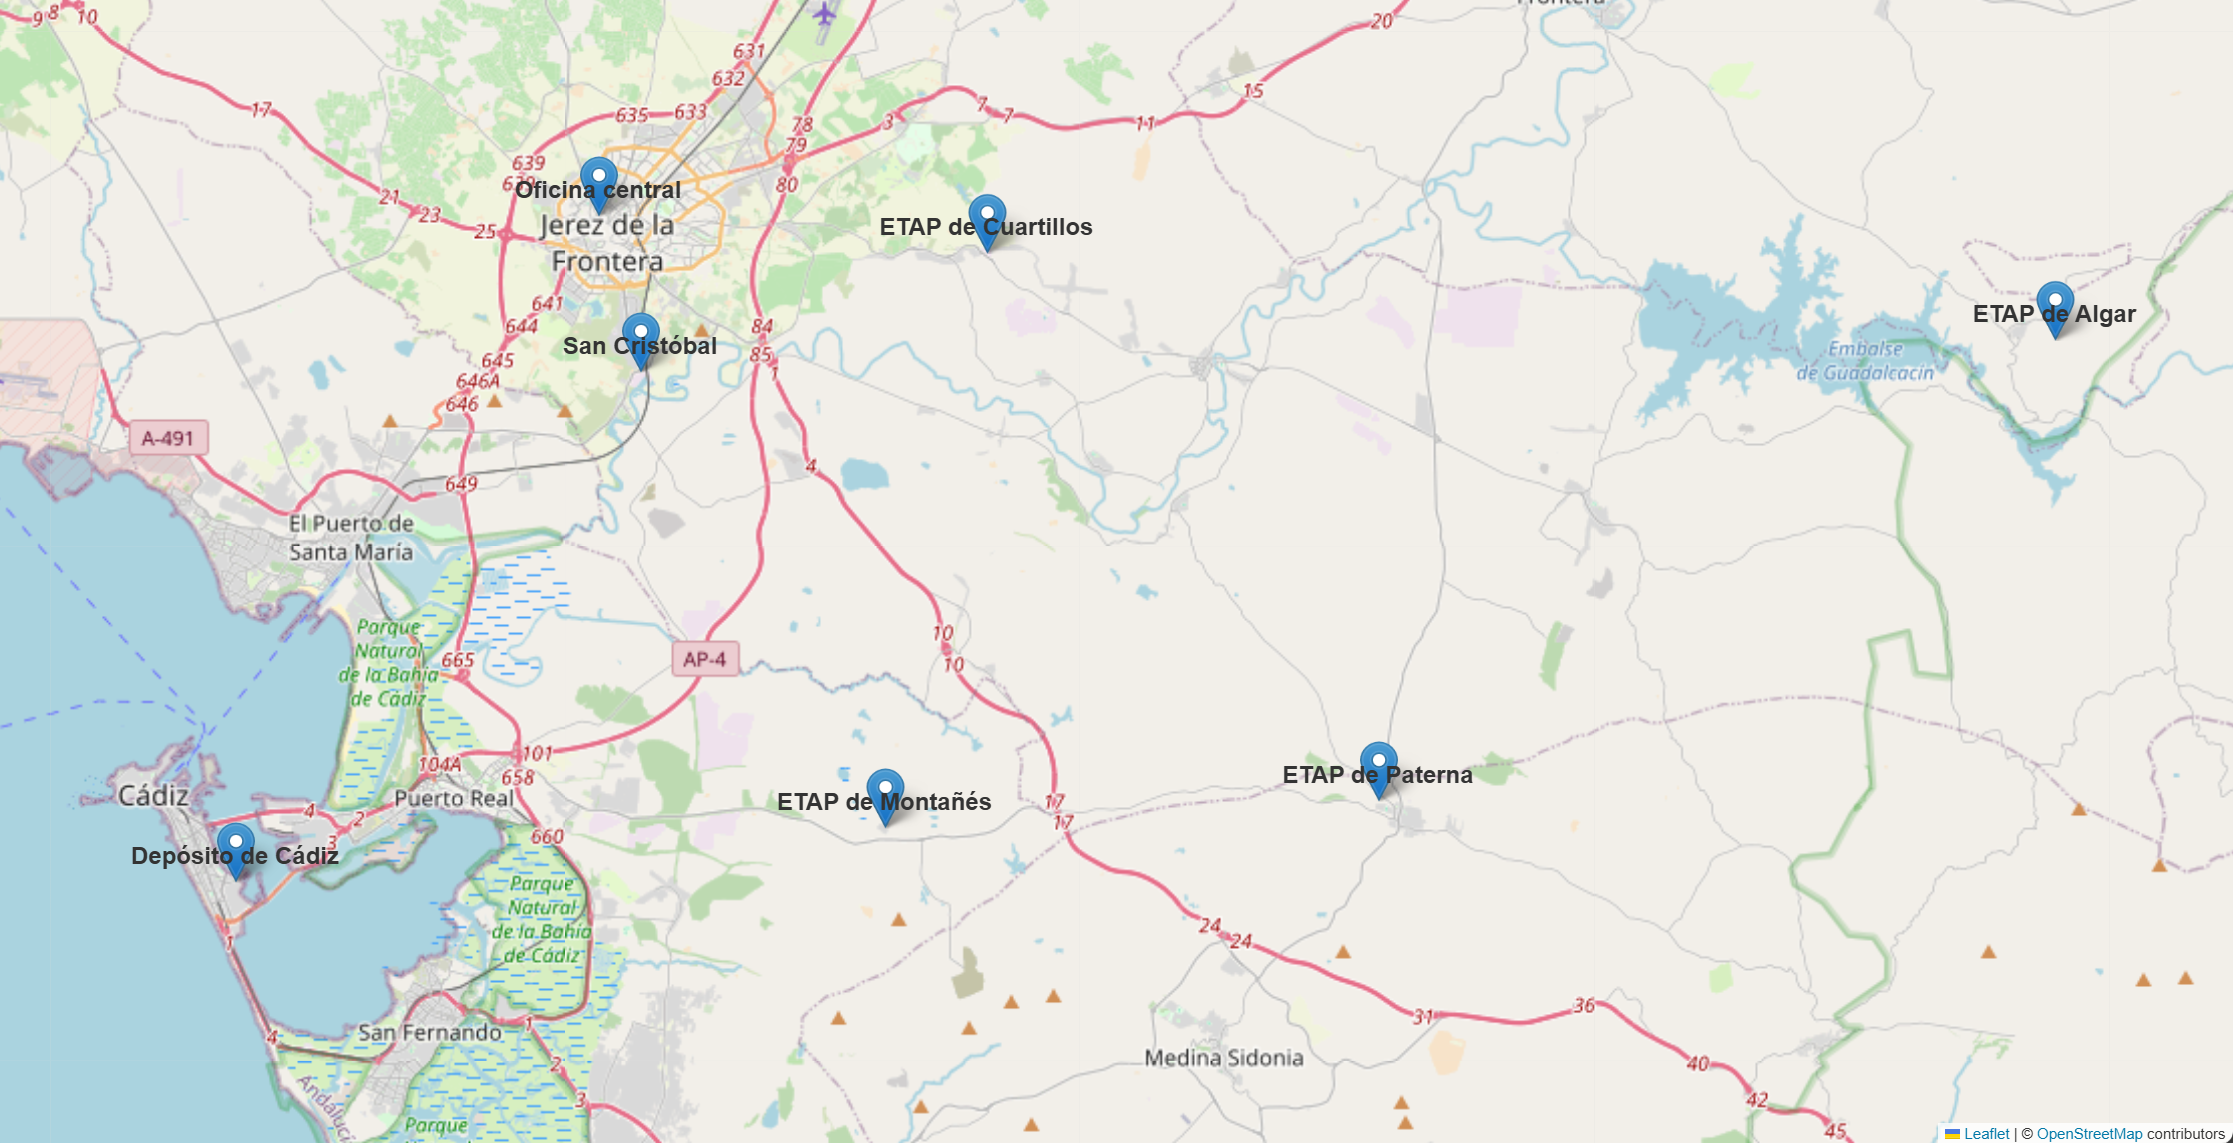
\includegraphics[width=0.95\textwidth]{images/mapa_sedes.png}
	\caption{Ubicación de las instalaciones}
	\label{fig:mapa_sedes}
\end{figure}

\subsection{SD-WAN (Software-Defined Wide Area Network)}
SD-WAN \cite{versa_sdwan} es una red de área extensa (WAN) que utiliza tecnología de redes definidas por software, ofreciendo servicios de red confiables y escalables. Esta tecnología permite simplificar el control y la administración de la infraestructura de red al proporcionar una arquitectura WAN virtual que conecta de manera segura a lo usuarios con las aplicaciones y servicios que necesitan. Asimismo, SD-WAN utiliza una combinación de tecnologías, como por ejemplo, MPLS, Internet de banda ancha y LTE, para ofrecer una conectividad flexible y de alto rendimiento. 

\vspace{0.5cm}
El funcionamiento de SD-WAN se basa en crear una superposición para virtualizar la red de área extensa, lo que permite un control centralizado, la simplificación de la administración y la implementación de los servicios de red.

\vspace{0.5cm}
\noindent
En cuanto a la arquitectura de este tecnología \cite{hpe_sdwan}, esta se compone de varios componentes clave, como:
\begin{itemize}
  \item \textbf{Dispositivos en el extremo:} son los dispositivos físicos o virtuales instalados en ubicaciones remotas, centro de datos y ubicaciones en la nube. Las cuales, tienen un rol importante como distribuir el tráfico según las políticas definidas y de medir en tiempo real el estado de la red.
  \item \textbf{Organizador de SD-WAN:} sirve para controlar las decisiones de política, como la gestión del tráfico y las rutas a utilizar.
  \item \textbf{Capa de transporte:} SD-WAN funciona con cualquier tecnología de transporte basado en IP, como MPLS, LTE, o 5G. Esta capa forma la red subyacente mientras que SD-WAN crea una red superpuesta inteligente con selección dinámica de rutas y conmutación de fallos. 
\end{itemize}

\subsection{MPLS (Multiprotocol Label Switching)}
\label{subsec:mpls}
MPLS (Multiprotocol Label Switching) \cite{wikipedia_mpls} es un mecanismo de transporte de datos que opera entre la capa de enlace de datos y la capa de red del modelo OSI. Este fue diseñado para unificar el servicio de circulación de datos para las redes basadas en circuitos y en paquetes. Asimismo, puede ser utilizado para transportar diferentes tipos de tráfico, incluyendo el de voz y el de paquetes IP.

\vspace{0.5cm}
\noindent
En una red MPLS existen diferentes elementos \cite{mpls_elements} que desempeñan distintas funciones en la red. En la Figura~\ref{fig:arquitectura_mpls} se puede observar una arquitectura de red MPLS típica.
\begin{enumerate}
  \item \textbf{Routers según ubicación y función en la red:}
  \begin{itemize}
    \item \textbf{Router del cliente (CE - Customer Edge):} es el router que se encuentra en el extremo del cliente. Puede ser cualquier router que se use para comunicarse con el proveedor de servicios.
    \item \textbf{Router de proveedor (PE - Provider Edge) o LER (Label Edge Router):} es el router frontera entre la red del cliente y la red MPLS del proveedor de servicios. Estos routers son los puntos de entrada y salida de la red MPLS.
    \item \textbf{Router troncal (P - Provider) o LSR (Label Switching Router):} es el router que se encarga de conmutar las etiquetas en el core de la red MPLS. Estos routers son responsables de dirigir el tráfico a través de la red utilizando las etiquetas asignadas. Además,
    intercambian estas etiquetas para dirigir el tráfico rápidamente a través de las red sin necesidad de analizar la dirección de destino de cada paquete. Su unión es puramente interno para el enrutamiento basado en etiquetas, por lo que no interactúan
    con los clientes.
  \end{itemize}
  \item \textbf{Otros elementos:}
  \begin{itemize}
    \item \textbf{LSP (Label Switched Path):} es el nombre genérico de un camino MPLS, es decir, es un túnel MPLS unidireccional establecido entre los extremos formado por un conjunto de LSRs.
    \item \textbf{LDP (Label Distribution Protocol):} es un protocolo para la distribución de etiquetas MPLS entre los equipos de la red.
    \item \textbf{FEC (Forwarding Equivalence Class):} es un grupo de paquetes tratados del mismo modo por el conmutador. Es decir, un conjunto de paquetes que se encaminan a través de la misma ruta en la red MPLS.
  \end{itemize}
\end{enumerate}

\begin{figure}[htb]
  \centering
  \includegraphics[width=1\textwidth]{images/Arquitectura_MPLS.png}
  \caption{Arquitectura MPLS}
  \label{fig:arquitectura_mpls}
\end{figure}

% MPLS se le conoce como un protocolo Layer 2.5, pues se encuentra entre la capa 2 (Enlace de datos) y la capa 3 (Red) del modelo OSI. Esto significa que MPLS puede trabajar con diferentes protocolos de red, como IP, Frame Relay y ATM, lo que lo hace muy versátil.

% \vspace{0.5cm}
%
% En la Figura~\ref{fig:mpls} se muestra una imagen de la cabecera de un paquete MPLS, que se compone de 4 campos, cada uno con un tamaño específico:
% La cabecera de un paquete MPLS se compone de 4 campos, cada uno con un tamaño específico:
% \begin{itemize}
%   \item \textbf{Label:} Es un campo de 20 bits que contiene la etiqueta de ruta utilizada para dirigir el paquete a su destino.
%   \item \textbf{CoS (Class of Service):} Es un campo de 3 bits que se utiliza para indicar la clase de servicio del paquete. Esto permite a los routers priorizar el tráfico según su importancia.
%   \item \textbf{S o BoS (Bottom of Stack):} Es un campo de 1 bit que se utiliza para indicar si la etiqueta es parte de una pila de etiquetas. 
%   \item \textbf{TTL (Time to Live):} Es un campo de 8 bits que se utiliza para indicar el tiempo de vida del paquete. Esto permite a los routers descartar paquetes que han estado en la red durante demasiado tiempo.
% \end{itemize}

% \begin{figure}[H]
%   \centering
%   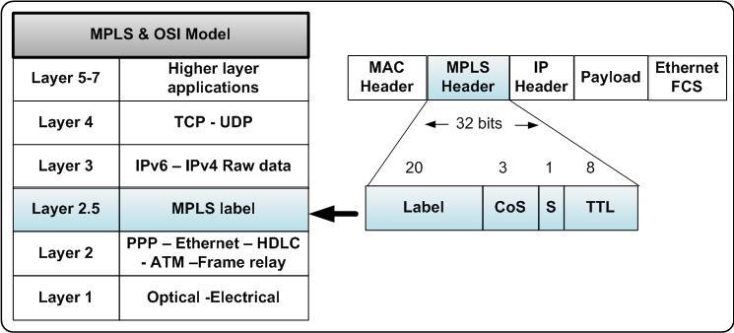
\includegraphics[width=0.9\textwidth]{images/MPLS-and-OSI-model.png}
%   \caption{Cabecera de MPLS, obtenida de \cite{mpls_elements}}
%   \label{fig:mpls}
% \end{figure}

\subsection{VPN (Virtual Private Network)}
\label{subsec:vpn}
Una VPN (Virtual Private Network) \cite{wikipedia_vpn} es una tecnología que garantiza una extensión segura de la red de área local (LAN) sobre Internet. Lo que permite establecer un enlace punto a punto con el uso de conexiones dedicadas, cifradas o la combinación de ambas. Existen diferentes arquitecturas VPN, cada una con sus propias características y casos de uso. A continuación, se describen las más comunes:

\begin{itemize}
  \item \textbf{VPN de acceso remoto:} permite a los usuarios conectarse a la red de la empresa desde ubicaciones remotas utilizando una conexión segura a través de Internet. Una vez conectados, tienen un nivel de acceso parecido al que tendrían en la red local de la empresa.
  \item \textbf{VPN punto a punto:} este esquema permite conectar dos redes remotas a través de Internet de forma segura, como si estuvieran en la misma red local.
  \item \textbf{VPN de sitio a sitio:} permite conectar múltiples redes remotas entre sí a través de Internet, creando una red privada virtual que conecta todas las sedes de la empresa.
  \item \textbf{VPN de extranet:} permite a socios comerciales o proveedores acceder de forma segura a recursos específicos de la red de la empresa.
\end{itemize}

\subsection{VoIP (Voice over IP)}
La tecnología VoIP \cite{voipstudio_que_es_voip} (Voice over IP) se refiere a la capacidad de realizar llamadas de voz a través de Internet en lugar de utilizar las líneas telefónicas tradicionales. Esencialmente, VoIP convierte las señales de voz en paquetes de datos que se transmiten a través de la red de Internet hasta llegar al destinatario, donde se convierten de nuevo en señales de voz.

\vspace{0.5cm}
VoIP ofrece varias ventajas sobre la telefonía tradicional, como costes más bajos en comparación con las tarifas de las líneas telefónicas convencionales, especialmente en llamadas de larga distancia e internacionales, e incluso suelen ser gratuitas o a un coste muy bajo. También, ofrece una mayor flexibilidad y escalabilidad, ya que permite añadir fácilmente líneas adicionales y funcionalidades avanzadas sin necesidad de instalar hardware adicional. Asimismo, permite la movilidad de los usuarios, ya que las llamadas pueden realizarse desde cualquier dispositivo con conexión a Internet.


\subsection{MP-BGP (Multiprotocol Border Gateway Protocol)}
MP-BGP (Multiprotocol Border Gateway Protocol) \cite{wikipedia_mp_bgp} es una extensión del protocolo BGP (Border Gateway Protocol) que permite distribuir en paralelo diferentes tipos de direcciones IP, como IPv4 e IPv6, además de, otros protocolos de red. Asimismo, utiliza una arquitectura básica con sistemas autónomos (AS) que se comunican a través de sesiones BGP e intercambian información de accesibilidad de red en forma de actualizaciones BGP \cite{linkedin_mp_bgp}. Estas se pueden clasificar en dos formas según el sistema autónomo (AS) al que pertenecen los routers que intercambian información de enrutamiento:

\begin{itemize}
  \item \textbf{iBGP (Internal BGP):} es la comunicación de routers del mismo sistema autónomo (AS) que intercambian información de enrutamiento.
  \item \textbf{eBGP (External BGP):} es la comunicación de routers de diferentes sistemas autónomos (AS) que intercambian información de enrutamiento.
\end{itemize}

Por otro lado, existen cuatro tipos de mensajes BGP \cite{wikipedia_bgp} que se utilizan para establecer y mantener las sesiones BGP:
\begin{itemize}
  \item \textbf{OPEN:} se utiliza para establecer una sesión BGP una vez haya sido establecido la conexión TCP.
  \item \textbf{UPDATE:} es un mensaje de actualización que contiene los anuncios de nuevos prefijos.
  \item \textbf{KEEPALIVE:} una vez la sesión BGP está activa, envía periódicamente un mensaje para mantener activa la conexión.
  \item \textbf{NOTIFICATION:} envía al cerrar una sesión BGP. Esto sucede cuando ocurre algún error.
\end{itemize}

\newpage

\section{Herramientas}
Las herramientas que se han utilizado para la realización de este proyecto son las siguientes:

\subsection{GNS3}
GNS3 (Graphic Network Simulator-3) \cite{gns3_wiki}, un simulador gráfico de red libre y de código
abierto que permite crear topologías de red complejas y poner en funcionamiento simulaciones sobre ellas, 
permitiendo así la combinación de dispositivos reales como virtuales.

\vspace{0.5cm}
Entre las principales características de GNS3 \cite{ccnadesdecero_gns3}, podemos destacar, que es un software gratuito y de código abierto, siendo disponible para Windows, Linux y macOS. De igual forma, no tiene límite en la cantidad de dispositivos que se pueden simular, a excepción de la limitación hardware: CPU y memoria. Además, permite la captura de paquetes de red con Wireshark, la conexión de redes simuladas con redes reales y está constantemente actualizado ya que cuenta con una comunidad de usuarios grande y activa (+800.000 usuarios).

\vspace{0.5cm}
Pero la ventaja principal es que los equipos de red simulados disponen de todas las funcionalidades de un equipo real, ya que ejecuta el mismo firmware que el equipo real. Permitiendo diseñar una topología de red simulada lo más parecida posible a una red real sin necesidad de tener los equipos físicos. 

\subsection{Wireshark}
Wireshark \cite{wikipedia_wireshark} es un analizador de protocolos utilizado para realizar análisis y solucionar problemas en redes de comunicaciones, para análisis de datos y protocolos, y como una herramienta didáctica.

\subsection{Docker}
Docker es \cite{docker_ubuntu_tutorial} una aplicación que simplifica el proceso de administración de procesos de software en contenedores. Estos permiten ejecutar aplicaciones en procesos con aislamiento de recursos. Son similares a las máquinas virtuales, pero son más portátiles, más flexibles con los recursos y más dependientes del sistema operativo host.

\subsection{VirtualBox}
Oracle VirtualBox \cite{virtualbox_introduction} es una herramienta de virtualización multiplataforma que permite ejecutar múltiples sistemas operativos simultáneamente en un mismo equipo físico, mediante la creación de máquinas virtuales (VM). Esta aplicación amplía las capacidades del sistema anfitrión, haciendo posible, por ejemplo, ejecutar distribuciones de Linux en un sistema Windows, o viceversa, así como combinar diferentes entornos como Windows 
y macOS o servidores Linux. 

\subsection{MicroSIP}
MicroSIP \cite{microsip} es un softphone de código abierto y portable, diseñado para sistemas operativos Windows y basado en la pila PJSIP. Esta herramienta permite realizar llamadas VoIP de alta calidad, tanto entre usuarios como hacia teléfonos convencionales, mediante el protocolo SIP (Session Initiation Protocol).

\subsection{Telefonos Grandstream GRP2601}
El teléfono Grandstream GRP2601 \cite{grandstream_grp2601_datasheet} es un modelo esencial de 2 líneas diseñado con aprovisionamiento zero-touch para implementación masiva y fácil gestión. Se caracteriza por tener un diseño elegante y un conjunto de funciones de última generación incluyendo conferencia de voz de 5 participantes para maximizar la productividad, soporte EHS para auriculares Plantronics, Jabra y Sennheiser y soporte en múltiples idiomas.

\subsection{Router Mikrotik RB2011UiAS-RM}
El router RB2011UiAS-RM \cite{mikrotik_rb2011uias_rm} de Mikrotik funciona con RouterOS, un sistema operativo de enrutamiento avanzado que ofrece funcionalidades como enrutamiento dinámico, hotspot, cortafuegos, MPLS, VPN, calidad de servicio, equilibrio de carga, supervisión en tiempo real y más. Este modelo destaca por sus cinco puertos LAN Gigabit, cinco puertos LAN Fast Ethernet, puerto serie RJ45, puerto USB, 128MB de RAM, licencia RouterOS L5 y pantalla LCD táctil para facilitar la configuración y gestión. 

\subsection{Switches TP-Link T2500G-10TS}
El T2500G-10TS \cite{tp_link_t2500g_10ts} es un switch gestionable con puertos Gigabit en todas sus interfaces, ideal para redes de alto rendimiento. Ofrece seguridad avanzada (IP-MAC-puerto, ACL, 802.1X, Radius, DoS, DHCP Snooping), QoS en L2/L3/L4 e IGMP Snooping para optimizar voz y video, y múltiples opciones de gestión (Web, CLI, Telnet, SSH, SNMP). Además, soporta funciones L2 como VLAN 802.1Q, QinQ, port mirroring y STP/RSTP/MSTP para una red estable y segura. 